\chapter{Conclusion}
    Sculptures have been precisely defined, by following the intuition of Pratt, as well as shown to be in close correspondence with ST-structures and Chu spaces. This nicely captures Pratt's event-state-duality.
    
    We have developed an algorithm to decide whether a higher-dimensional automaton is a sculpture, and it has been used to show that, unexpectedly, some quite simple acyclic higher-dimensional automata are not sculptures. In Theorem \ref{th:non-sculpting}, we showed that a higher-dimensional automata is a sculptures, however, its unfolding is not a sculpture. We believe that this contradicts Pratt's intuition that sculptures suffice for modelling of concurrent behaviour. We may present the results of this thesis by the diagram below:
    
    \begin{center}
        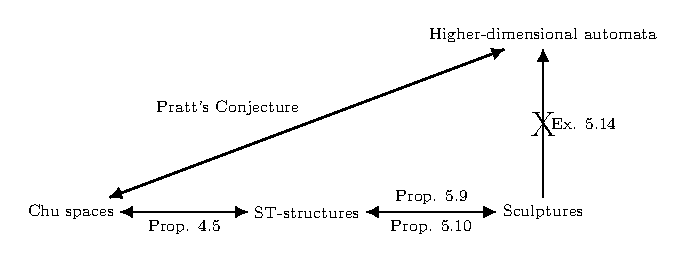
\includegraphics[scale=1]{Figures/4.Relationship-with-other-models-of-concurrency/Chu-spaces-and-ST-structures/argument-diagram.pdf}
    \end{center}
    
    In Proposition \ref{prop:ST-structure-Chu-over-3}, we showed the isomorphism between Chu spaces and ST-structures. In Proposition \ref{prop:ST-to-Sculpture} and Proposition \ref{prop:Sculpture-to-ST}, we show that ST-structures and sculptures are isomorphic. Hence, sculptures are also isomorphic to Chu spaces. To strengthen the proofs, we provided examples of higher-dimensional automata which are not sculptures, see Example \ref{exp:hda-broken-box}. We used this example to show the \emph{non-sculpting} theorem.
    
\section*{Future work}
    In this thesis, we presented combinatorial sculpting and is not to be confused with \emph{geometric} sculpting which consists of taking a geometric cube of some dimension and chiseling away hypercubes which one does not want to be part of the structure.
    
    Geometric sculpting has been used by Fajstrup et al. in~\cite{Fajstrup06AlgebraicTopologyConcurrency, Fajstrup98detectingdeadlocks, Fajstrup16DirectedAlgebraicTopologyConcurrency} and other papers to model and analyze so-called PV programs: processes which interact by locking and releasing shared resources.  In the simplest case of linear processes without choice or iteration this defines a hypercube with \emph{forbidden hyperrectangles}, which cannot be accessed due to resources access limits.  See Fig.~\ref{fig:swiss} for an example.
    
    \begin{figure}[ht]
        \centering
        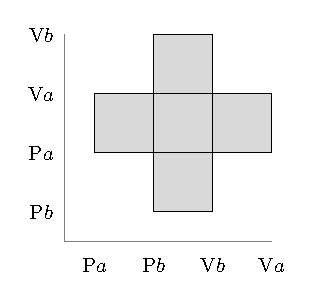
\includegraphics[scale=1.2]{Figures/6.Conclusion/swiss.pdf}
        \captionof{figure}[Swiss flag]{Two PV processes sharing two mutexes.  The forbidden area is
    grayed out.}
        \label{fig:swiss}
    \end{figure}
    
    Technically, geometric sculptures are \emph{Euclidean cubical complexes}; rewriting a proof in \cite{Ziemianski17} will show that such complexes are precisely (combinatorial) sculptures. This will be presented in a current paper, which is being submitted to FOSSACS 2019. Hence, higher-dimensional automata is Euclidean iff it is a sculpture, so that the geometric models for concurrency~\cite{Fajstrup06AlgebraicTopologyConcurrency, Fajstrup98detectingdeadlocks, Fajstrup16DirectedAlgebraicTopologyConcurrency} will show to be closely related to the combinatorial ones~\cite{pratt91hda, Glabbeek91BismiluationHDA}, through the notion of sculptures. Much work has been done in the \emph{geometric} analysis of Euclidea higher-dimensional automata~\cite{FajstrupRGH04FundCatI, GoubaultH07FundCatII, Fajstrup98detectingdeadlocks, MeshulamR17, RaussenZ14, Ziemianski17}; by the equivalences of the current work being done in the FOSSACS paper, these results will be made available for combinatorial models.
    
    As we briefly introduced in Section \ref{sec:higher-dimensional-automata}, the notion of \emph{unfolding} 
    % is important in relation to sculpting.
    % Unfolding 
    removes iteration and is commonly used to turn a complicated model into a simpler, but potentially infinite one.
    % %  (e.g., operational finite state automata vs.\ denotational event-based models). 
    % It is thus, perhaps, expected that there are simple HDA which cannot be sculpted,
    % but their unfoldings can, see Fig.~\ref{fig:unfoldings} for two examples.
    It is thus expected that even if a higher-dimensional automata cannot be sculpted, its unfolding can, as illustrated by the two simple examples in Fig.~\ref{fig:unfoldings}.
    
    \begin{figure}[tbp]
        \centering
        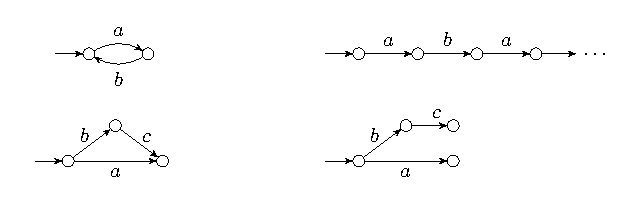
\includegraphics[scale=1.2]{Figures/6.Conclusion/unfolding.pdf}
        \captionof{figure}[Unfolding of two simple HDA]{Two simple HDA which cannot be sculpted (left) and their unfoldings (right) which can.  (The top-right sculpture is infinite.)}
        \label{fig:unfoldings}
    \end{figure}
    
    However, it can be shown that this is not the case, as witnessed by the example in Figure \ref{fig:speedAngelDemon}  which shows a higher-dimensional automaton which cannot be sculpted and which is its own unfolding. This example features two agents, $a$ and $d$, which compete to choose between two future events $b$ and $c$.  If the demon finishes his $d$ event first, then 
    % he imposes his choice between $b$ and $c$ (which he already has made before executing his $d$ event); 
    the choice between $b$ and $c$ is a demonic choice, that is, already made when starting the $d$ event;  if the angel finishes her $a$ event first, then 
    % she can freely choose between $b$ and $c$. 
    we have an instance of an angelic choice between $b$ and $c$. This system, introduced in~\cite{Johansen16STstruct}, cannot be modeled as a ST-structure, but \emph{can} be modeled as a ST-structure with \emph{cancellation}~\cite[Section~5]{Johansen16STstruct}.
    
    \begin{figure}[tbp]
        \centering
        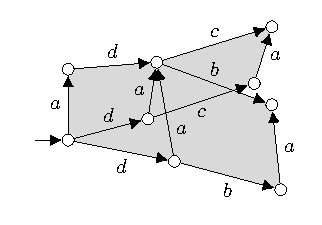
\includegraphics[scale=1.2]{Figures/6.Conclusion/angelicvsdemonic.pdf}
        \captionof{figure}[Speed game of "angelic vs. demonic choice"]{The HDA from~\cite{Johansen16STstruct} of the "speed game of angelic vs.\ demonic choice".}
        \label{fig:speedAngelDemon}
    \end{figure}

    Even more worrying is the fact that there are (acyclic) HDA which can be sculpted, but their unfoldings cannot; in fact Figure ~\ref{fig:HDA-broken-box}, is one such example. We showed, in Theorem \ref{th:non-sculpting}, that the unfolding did not return a simpler model, and which seems to contradict Pratt's claim that sculpting suffices for modeling.
    
    In the geometric setting, it can be shown that there are Euclidean cubical complexes whose unfoldings are not Euclidean.  Since Goubault-Jensen's seminal paper~\cite{Goubault92homologyof}, \emph{directed topology} (or \emph{ditopology}) has been developed in order to analyze concurrent systems as geometric objects~\cite{Grandis09book, Fajstrup06AlgebraicTopologyConcurrency, Fajstrup16DirectedAlgebraicTopologyConcurrency}.  Directed topology has been developed largely in analogy to algebraic topology, by \emph{breaking [its] symmetries}~\cite{Grandis09book}, but as shown time and time again, there are unexpected problems turning up.

    The mismatch being discovered in the current FOSSACS paper, between Euclidean complexes and unfoldings, is again such an unexpected problem.  Unfoldings of higher-dimensional automata have been developed as a directed analogue to \emph{universal covering spaces} in algebraic topology~\cite{Glabbeek91BismiluationHDA, Fahrenberg05PhD}, building a universal \emph{dicover} by considering dihomotopy classes of directed paths.  There are several other problems with this notion, for example it does not behave well under change of base point, and finding better definitions of dicovering is active ongoing research, see for example~\cite{jeremy18TreesPartialHDA}.
    
    We may sum up the claims being made here and in the FOSSACS paper as follows:
    
    \begin{enumerate}
        \item There are acyclic $\HDA$ which cannot be sculpted.
        \item There is a $\HDA$ which cannot be sculpted, but whose unfolding can be sculpted.
        \item There is a $\HDA$ which can be sculpted, but whose unfolding cannot be sculpted.
        \item There is a $\HDA$ which can be sculpted, but whose unfolding can be sculpted.        
    \end{enumerate}
    
    For future work of sculptures and unfoldings of $\HDA$, we would like to apply our decision algorithm to each of the mentioned cases. This thesis has already shown (3) as part of the \emph{non-sculpting} theorem.

    